\setcounter{section}{0}
\setcounter{figure}{0}
\setcounter{table}{0}
\newpage
\textbf{\LARGE{{Part two: Analysis, discussion and reflection}}}\\

Part two of this report explores the question of \textit{why}
the design process occurred as it did. In section~\ref{sec:participatory}
we consider what a design process is, in section~\ref{sec:overview}
we provide a general description of techniques used in the design process,
in section~\ref{sec:process} we describe how the authors realized an IT design
project using the \must{} method and in section~\ref{sec:detailed} we
look at a few of the key choices and techniques that were employed while working
on the design report.

The reader is expected to be familiar with details about \gomonkey{} 
from ``Part one: Design Project''.

\section{Participatory design in IT} \label{sec:participatory}
IT projects vary widely in size, shape and form. From the potentially small,
painless setup of Google Apps for a company of 3 employees, to the large-scale
migration of Jyske Bank's IT infrastructure after 2 years of
planning\cite{jyskebank}. This makes the task of providing \textit{generic}
advice a difficult one. A large portion of the work done in this report is based
upon the practices and techniques of participatory design as proposed by
\cite{bodker2004participatory}.  B\o dker et al.\ describe a search for
techniques, concepts and ideologies which may apply to the \textbf{design and
planning} of IT projects on a general level. 

Karat\cite{karat1997evolving} describes the active involvement of users as, ``We don't consider
usability as limited to the display and keyboard interface between human and machine, but rather
we recognize that it encompasses how any artefact fits into a complex work or home environment''.
Kujala\cite{kujala2003user} proposes that user involvement is most efficient and influential in the 
\textbf{early} stages of system development, as the cost involved in making changes increases during 
system development. These articles are some of several that support the notion of approaches such as 
participatory design\cite{bodker2004participatory} and contextual design\cite{beyer1997contextual}.

We define an \textbf{IT design project} here according to B\o dker et al.\ 
%%
\vspace{5mm}
\begin{framed}
    \textbf{IT design project}: A project conducted at a company that reveals
    goals, defines problems, and indicates solutions, with the aim of designing
    sustainable uses of IT based on a specific problem within the company.\cite{bodker2004participatory}
\end{framed}
\vspace{5mm}
%%
The \must{}\cite{bodker2004participatory} method consists of
\begin{inparaenum}[1)]
    \item an initiation phase
    \item an in-line analysis phase
    \item an in-depth analysis phase and
    \item an innovation phase.
\end{inparaenum}
It seeks to provide a perspective on IT design where you view IT projects not
just through the lens of what a prospective client wishes done, but also take into
account the work environment, the organization as a whole, the interaction
between company and customers and subsequent changes and impacts that making
alterations to a work environment can result in. This can be considered as an 
\textbf{ethnographic approach} to design.

The goals of participatory design are rooted in four guiding \textbf{principles}.
\begin{description}
    \item [The principle of a coherent vision] is concerned with making sure that stakeholders
        and employees come together in a joint venture to innovate, with the aim
        of providing a coherent vision of the future. There are several
        important points to this; a vision for change is not just a single IT
        system or implementation, but is a part of a whole that encompasses the
        organization, the employees, the work practices, the technology and
        systems. 
    \item [The principle of genuine user participation] is about using mutual learning activities
        to teach employees about technical options, issues and solutions and to
        teach the designers about the work that the employees are doing. There are
        two central goals that arise from this: increasing the chance that a
        finished system reflects \textbf{actual} work practices and
        requirements and increasing the chance that a finished system is used
        according to its original intentions.
    \item [The principle of firsthand experience with work practices] realizes that being told
        about how something occurs is not the same as reading about it, nor is
        it the same as actually experiencing the practice first-hand. All three
        approaches are applicable and should occur in a design project, but
        there may be factors influencing a re-telling of work practices or a
        written description that only surface during first-hand experience such
        as an interview, an observation or a think-aloud experiment.
    \item [The principle of anchoring visions] views the design process as a mutual learning
        process between all members of the project group, in order to gain a
        common understanding of the results produced by the design
        project\cite{bodker2004participatory}. Anchoring is about motivating,
        about making all participants in the design process \textbf{care}. This
        serves both to help eliminate misunderstandings and uncertainty
        that employees or management may have about proposed changes, instead
        transforming uncertainties into a positive work atmosphere aimed at
        improvement and innovation. The importance of this factor is underlined
        by other research such as \cite{standish20012}, who list the emotional
        maturity and ecosystem of the project as one of the most important
        components of successful IT projects.
\end{description}

The purpose of an IT design project is \textbf{not} to end up with a
finished implementation or actual, implemented alterations to company work
practice, but to provide a report that allows a company to make an
\textbf{informed choice} about a specific strategy or implementation plan to
adopt. Such a choice is an exercise in risk management. In 1995, The Standish
Group found the top four reasons for project success were user involvement,
executive management support, clear statement of requirements and proper
planning\cite{standish1995chaos}. Conversely, the top four reasons for failure
were found to be incomplete requirements, lack of user involvement, lack of
resources and unrealistic expectations respectively\cite{standish1995chaos}.
They also found that only about \textbf{19\%} of IT projects succeeded on-budget
and on-time\cite{standish1995chaos}. These kinds of failures are often
accompanied by a very real, costly risk.  In 2005, Bronte-Steward proposed that
approximately \$500 billion was wasted worldwide each year on IT purchases that
failed to reach their objectives\cite{bronte2005developing}. In 2006, the number
of successful projects as measured by The Standish Group\cite{standish2012} had
increased to \textbf{37\%}, attributed in part to the same four factors of
success as they had proposed in 1995. 

One avenue for moving towards better project success rate, is to focus on
improving the \textit{implementation} stage of software projects and improve the
development process itself, e.g.\ the innovation of methods such as agile
development. Another is to focus on the \textit{planning} stage of software
projects, which is what \must{} and this report concern themselves with, not
only to prevent failure but to provoke success.

Readers are encouraged to read \cite{bodker2004participatory} for a more
wholesome description of how the \must{} method works.

\section{Overview of techniques employed} \label{sec:overview}
The \must{} method describes 16 specific techniques that can be used, depending
on the phase of the project. Each technique serves a specific purpose, in that it
has pros and cons as far as information gathering, information organization or discovery
is concerned. Some techniques apply to specific phases of the \must{} method, and others
are relevant throughout the lifetime of the design project.

The activities listed below took place during the design project.
\begin{description}
    \item [Market study]: Market studies aim to clarify the current state of a
        domain, by doing research on competitors, market maturity and similar.
        As an activity it has broad application, in this report we are more
        specifically concerned with market studies of standard IT systems that
        provide a certain kind of functionality, namely booking.
\end{description}

The techniques listed below were used in the design project.
\begin{description}
    \item [Baseline Planning] The division of work into a series of phases,
        each of which is separated by a baseline (e.g.\ a milestone), that has well-defined
        requirements or goals. An initial set of baselines is produced during the initiation
        phase, which is then re-evaluated and detailed further as steps are completed and new
        baselines reached. The technique dates back to \cite{andersen1990professional}, and is
        analogous to planning a project in terms of milestones, goals and actionable items. This
        particular technique is a recurring task of the entire design project.

    \item [In-situ interview] Interviews are one of the most frequently used techniques in IT 
        design, particularly qualitative interviews\cite{bodker2004participatory}. An in-situ
        interview is one that occurs \textit{at} the workplace, as opposed to occurring at a
        remote location away from the work environment. The purpose of such an interview is often
        to clarify current work practice, tasks and function. Interviews are often transcribed as-is
        or summarized into a list of points.

    \item [Observation] An observation provides first-hand experience of
        concrete work practices, either that of the existing workflow or of a
        prototype or newly implemented system. Observation is a potentially
        time-consuming task, and care must be taken about how and what to record
        or transcribe as the immediate result of the observation. Observations
        can thus result in either video, audio or text, depending on what makes
        sense.

    \item [Diagnostic Mapping] A diagnostic map focuses on problem areas, causes
        of those problems, their consequences and subsequently one or more
        proposals for solutions. This technique applies primarily to the
        in-depth analysis phase, to relate problems and solutions in an
        easy-to-read fashion. Each row in a diagnostic map potentially
        represents a story that can be read using narrative such as, '\textbf{X}
        is a problem, caused by \textbf{A},\textbf{B} and \textbf{C}, having the
        consequence of \textbf{F}. So we should solve \textbf{X} by doing
        \textbf{Y}'. 

    \item [Think-aloud experiment] A think-aloud experiment is one in which a
        subject performs a series of tasks while expressing as much of their
        decision process as they can. The purpose is often to gain insight into
        the \textit{reasons} for performing actions or for continuing down a
        certain path of action. One possible application is to gain first-hand
        insight into current work practices.

    \item [Document analysis] A lot of potentially interesting and relevant
        information is often \textit{hidden away} in documents that occur as
        part of a work practice. Permission slips and responsibility waivers,
        booking forms and so on. Document analysis aims to extract pertinent
        information from one or more documents that are part of the work
        practice. For example, annual reports and organizational diagrams may
        help tell the design group about the company as a whole, while specific
        documents used as part of a task may help shed light on the way that
        task occurs and the flow of information either inside the company or
        between customer and company.

    \item [Developing scenarios] This technique dates back to at least
        \cite{clausen1993narratives} and revolves around creating prose-style
        representations exemplifying a certain work practice, under future use
        of the system. This both anchors employees and helps develop a coherent
        vision of the future for all participants of the design group. A more
        common name for this technique is possibly the development of
        \textit{user stories} or \textit{usecases}, which embody a similar if
        not the same intent.

    \item [Experimenting with prototypes] A horizontal
        prototype\cite{bodker2004participatory} is one which has no real
        functionality, such that any functionality or interaction with the
        prototype must be \textbf{simulated} (e.g.\ a paper-based mockup
        prototype). A vertical prototype\cite{bodker2004participatory} is one
        that has functionality and is based in a real IT-based solution that
        functions, at least partially. Experimenting with a prototype can
        provide valuable information, either in a structured manner by walking
        through specific usecases, or as a more workshop-oriented approach where
        a model is examined and discussed in plenum for benefits of
        brainstorming, correcting misunderstandings and more. The technique also
        helps anchor employees.
\end{description}

\section{From beginning to end: The design process} \label{sec:process}
The following is written in a narrative style, as the purpose is to
walk the reader through the sequence of events as they occured from one
to the next. To avoid mixing reflection and an account of things that happened,
the narrative is split into a section for each phase followed by reflection on
that particular phase.

\subsection{The initiation phase}
\gomonkey{} was contacted by the authors because they had a contact at the
company and the website \url{www.gomonkey.dk} showed obvious issues with
regards to the booking system. Suspicions were confirmed over the telephone,
where the owner and manager at \gomonkey{}, Michel, agreed to an initial in-situ
meeting. The meeting was to establish grounds for a design project, focused on
the booking system of the \gomonkey{} website. A qualitative, unstructured
in-situ interview was conducted between two of the authors and Michel, to
introduce the prospect of a design project, to establish a common level of
expectation and to verify the problem first-hand. Notes were taken on paper
during the interview, which were later transcribed into a summary of points that
described: the managers description of customer bookings, the managers
description of his own workflow, the existing IT infrastructure of \gomonkey{},
the company organization, a list of competitors and minor notes on auxiliary
nice-to-have ideas.

Based upon this summary of points, a document with project description and
specification were drawn up, along with an initial baseline plan. The project
specification included information on existing IT infrastructure, the skill-set
of the design team (the authors) and a list of stakeholders and participants.

\reflection{}
%%%%
\begin{description}
    \item [Choice of interview form] As \cite[p.228]{bodker2004participatory} describes,
        an unstructured interview form is often used for qualitative interviews,
        where dialog is a desired by-product and conversation can stray across a
        broad range of topics. This is in stark contrast to a more structured
        interview, which may have been more appropriate if it was possible to line 
        up all of the employees and ask specific questions about the existing IT
        system and workflow.

    \item [Length of initiation phase] The initiation phase was quite short in this instance.
        While the initial scope of the project was always supposed to be the
        booking system, the initiation phase failed to clarify on important
        aspects of the project, such as whether auxiliary systems like payment 
        would be considered part of the design project. In addition, where
        \cite{bodker2004participatory} recommends signing a project charter
        between the design team and the stakeholders, no such charter was
        signed. This prevented a potential avenue for anchoring the employees,
        and left the ball in the design teams court, so to speak. Precisely
        because the project was on a short deadline, making sure to clearly
        establish scope from the get-go could have had an important effect on
        how the remaining time was spent.

    \item [Building a baseline plan] The initial interview with the manager
        provided the basis for the construction of a baseline plan. As
        \cite{bodker2004participatory} notes, such a plan is initially quite
        vague, gaining in specificity as the project ages and matures. Enough
        information was uncovered during the interview to successfully create a
        baseline plan, even if that information would be invalidated at a later
        stage when uncovering new information.
\end{description}

\subsection{The in-line analysis phase}
The purpose of the in-line analysis phase was to establish a more thorough
understanding of any IT strategy the company already had, gauge how \gomonkey{}
employees and management viewed the current IT situation and to narrow the scope
with regards to the work domains that the design project would cover. Much of
this was already covered initially in the initiation phase, as part of the very
first interview that took place with the manager, Michel. An additional
unstructured interview was conducted with an employee, Nanna. The interview was
recorded as an audio file and later transcribed to a text file of summarized
points, and together with prior knowledge from the initiation phase formed the
basis of a document covering the in-line analysis phase. In particular, the
document described a list of potential business processes, a bullet-point list
describing the environment, a prioritized business strategy, a list of IT
systems and a list of relevant work domains. 

\reflection{}
%%%%
\begin{description}
    \item [In-line analysis as a phase] Normally, this phase is marked by a
        high level of cooperation and communication between the company and the
        designers\cite{bodker2004participatory}. However, looking at
        \cite[p.120, Figure 5.1]{bodker2004participatory}, the \gomonkey{}
        design project was estimated to be in \textbf{``Situation 2''}, that is,
        a routine situation under which there was no pre-existing IT strategy
        and the problem was clarified from the get-go. The in-line analysis
        phase would have ideally occurred as a simple activity in the initiation
        phase, covering a process similar to \cite[p.131, Figure
        5.3]{bodker2004participatory} in order to map out the relationship
        between environment, strategy, processes, work domains and the resulting
        IT systems. Unfortunately, course requirements forced it to be a separate phase
        altogether. 
    \item [Unstructured interview with Nanna] The unstructured form makes sense for the
        in-line analysis and \gomonkey{}, as the intent was to cover a number of
        different topics and lead the interviewed to describe, with their own
        words and in their own way, a number of different things related to the
        work practice and perception of IT systems.
\end{description}

\subsection{The in-depth analysis and innovation phase}
The starting point for the in-depth analysis and innovation phase was the
identified work domains, IT systems and business goals from the in-line
analysis.  To gain a more in-depth understanding of how booking at \gomonkey{}
worked and clarify work practices in general, a number of techniques were used:

\begin{description}
    \item [Meeting] A meeting was held
        between the manager, Michel, and the design team. The meeting was
        focused entirely on the booking process as a work domain, in an attempt
        to sketch out corner cases, understand the flow of communication between
        \gomonkey{} and customers and employees, identify paper documents that
        would be part of the process and most importantly understand the
        \textbf{reasons} for the current work practice functioning as it does.
        The result of the meeting was a text transcription of summarized points
        and identified key documents, which were slated for a document analysis
        at a later point in time. 

    \item [Document analysis] The documents identified in the meeting were
        analyzed. One of the documents were a description of the procedure
	which an instructor has to perform, and this clarified a part of the
	handling of customers which we were not aware of at the current time. 
	The same point was later encountered in an observation, so the results 
	from the document analysis were not exceptionally revealing.

    \item [In-situ Observation] An in-situ observation of the manager was performed,
        to observe three different work processes: 
        \begin{inparaenum}[1)]
            \item how the manager handles receiving a booking
            \item how the manager checks the payment status of a booking
            \item any work processes that occur prior to a booking arriving.
        \end{inparaenum}
        Almost no preparation took place to facilitate the observations, beyond
        coming up with what cases to specifically observe. The observations
        occured in-situ at \gomonkey{}. The design team contacted Michel by
        phone and agreed on two times which the observations could occur, and
        each observation was then filmed with a smartphone. The observations
        helped clarify the workflow from the managers point of view, although
        the third observation provided little to no information transferable
        into an IT system context. \autoref{fig:michel_obs} shows a still from
        the observation of the manager answering an e-mail in relation to a
        booking. \autoref{fig:calendar} shows a still image of the managers
        calendar, being checked to make sure a booking is possible.

        \begin{figure}
            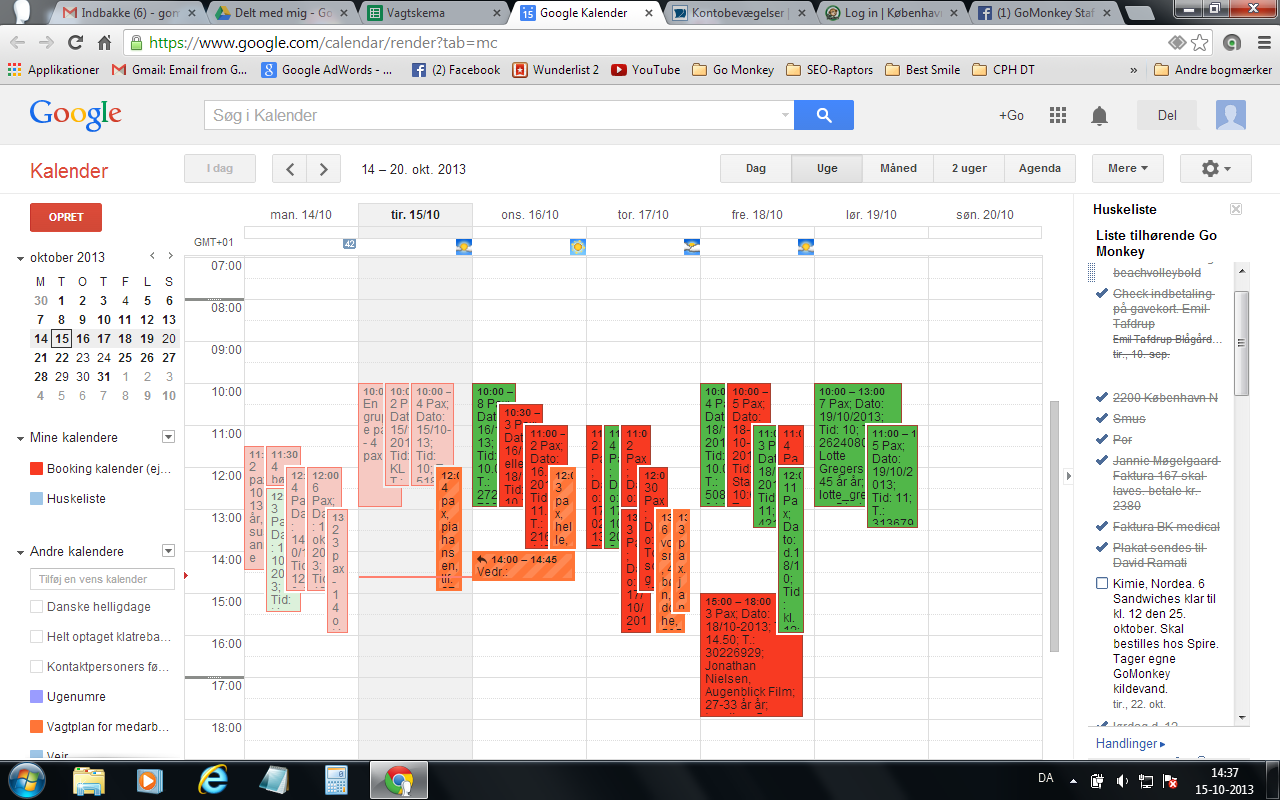
\includegraphics[width=\textwidth]{figures/calendar}
            \caption{The booking calendar of \gomonkey{ }. \label{fig:calendar}}
        \end{figure}

        \begin{figure}
            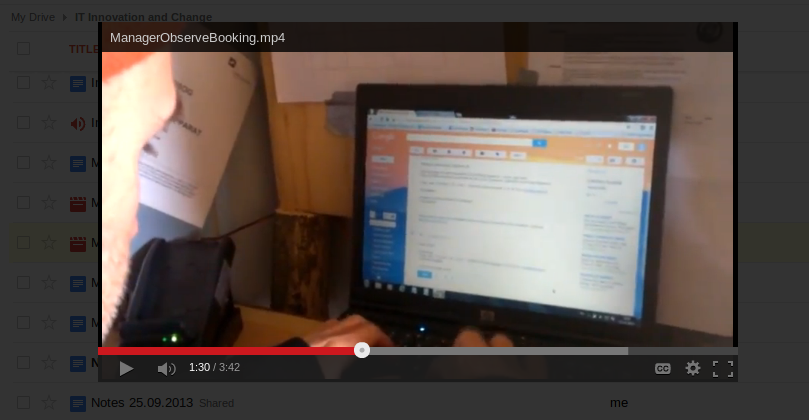
\includegraphics[width=\textwidth]{figures/observation}
            \caption{The manager of \gomonkey{ } responding to a customer e-mail
            about a booking. \label{fig:michel_obs}}
        \end{figure}

    \item [Think-aloud experiment] A think-aloud experiment was constructed for
        a potential customer, focused around the booking work flow. The
        potential customer is a friend of a member of the design team, a scout
        leader contemplating booking a trip for his scouts. The
        experiment took place in the subjects own apartment and was recorded on
        video through a smartphone. The only setup required by the design team
        was to decide in advance that the user should try and perform a booking
        through the \gomonkey{} website. The video was later described in a text
        document, describing the circumstances of the experiment and its
        results. The experiment shed light on many of the initial concerns the
        design team had with the existing booking form, confirming several of
        the issues that were found with it. Four things in particular were
        highlighted as problems, by the subject: bad response from submission of the form,
        lack of e-mail confirmation, problematic entering of booking date,
        pre-entered text was a nuisance. \autoref{fig:cust_obs} shows a still
        taken from a video of the think-aloud experiment.

        \begin{figure}
            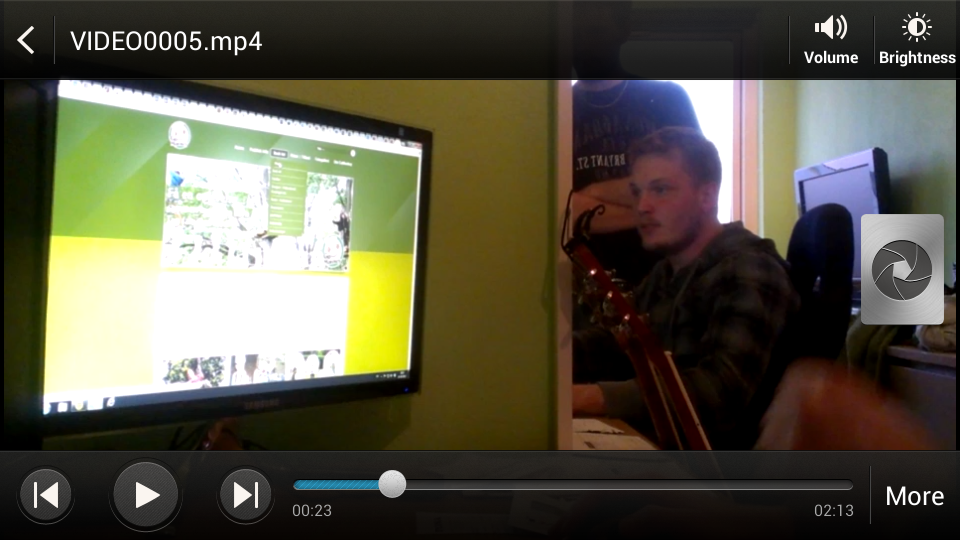
\includegraphics[width=\textwidth]{figures/cust_observe}
            \caption{A customer logs onto \url{www.gomonkey.dk} to make a
            booking. \label{fig:cust_obs}}
        \end{figure}
    \item [In-situ interview] An in-situ interview with the manager was
        performed, which took on a structured format and was focused on how the
        Manager handles scheduling employee work schedules. In this interview,
        it was revealed that there is a simple phone-list and the Manager has an
        idea of which employees can handle larger groups of customers easily and
        which cannot. Interaction with some employees occurs via mail, some via
        SMS, some via a phone call. If one employee cannot come, then the next
        on the list gets called, and so on. For the manager, a system to
        schedule employee times is not of huge priority, because the existing
        system works and he believes both the employees and himself are happy
        with it.
    \item [Diagnostic Map] The design team created a diagnostic map, based on
        problems identified throughout the interviews and observations performed 
        during the in-depth analysis phase. Particular attention was paid to
        problems related to work processes. As such, it reflects the view of the
        current problems, effects and potential solutions that the design team
        had at the time of its creation. This also means that the diagnostic map
        was \textbf{not} used as an anchoring device\cite{bodker2004participatory}, 
        as \gomonkey{} had no part in its creation. 
\end{description}

Based upon the results of the aforementioned techniques, prioritized goals and
problems were scoped out. This served to simplify subsequent work with the
limited time we had available and assist in making prioritized choices about how and
where to innovate. Importantly, the techniques covered enough ground for us to
begin the innovation aspect with the new-found knowledge, documented as an
analysis report\cite[p. 159]{bodker2004participatory} that describes backdrop
and focus, goals, problems, needs, ideas for solutions as well as suggested
priorities through means such as a diagnostic map.

\begin{figure}
    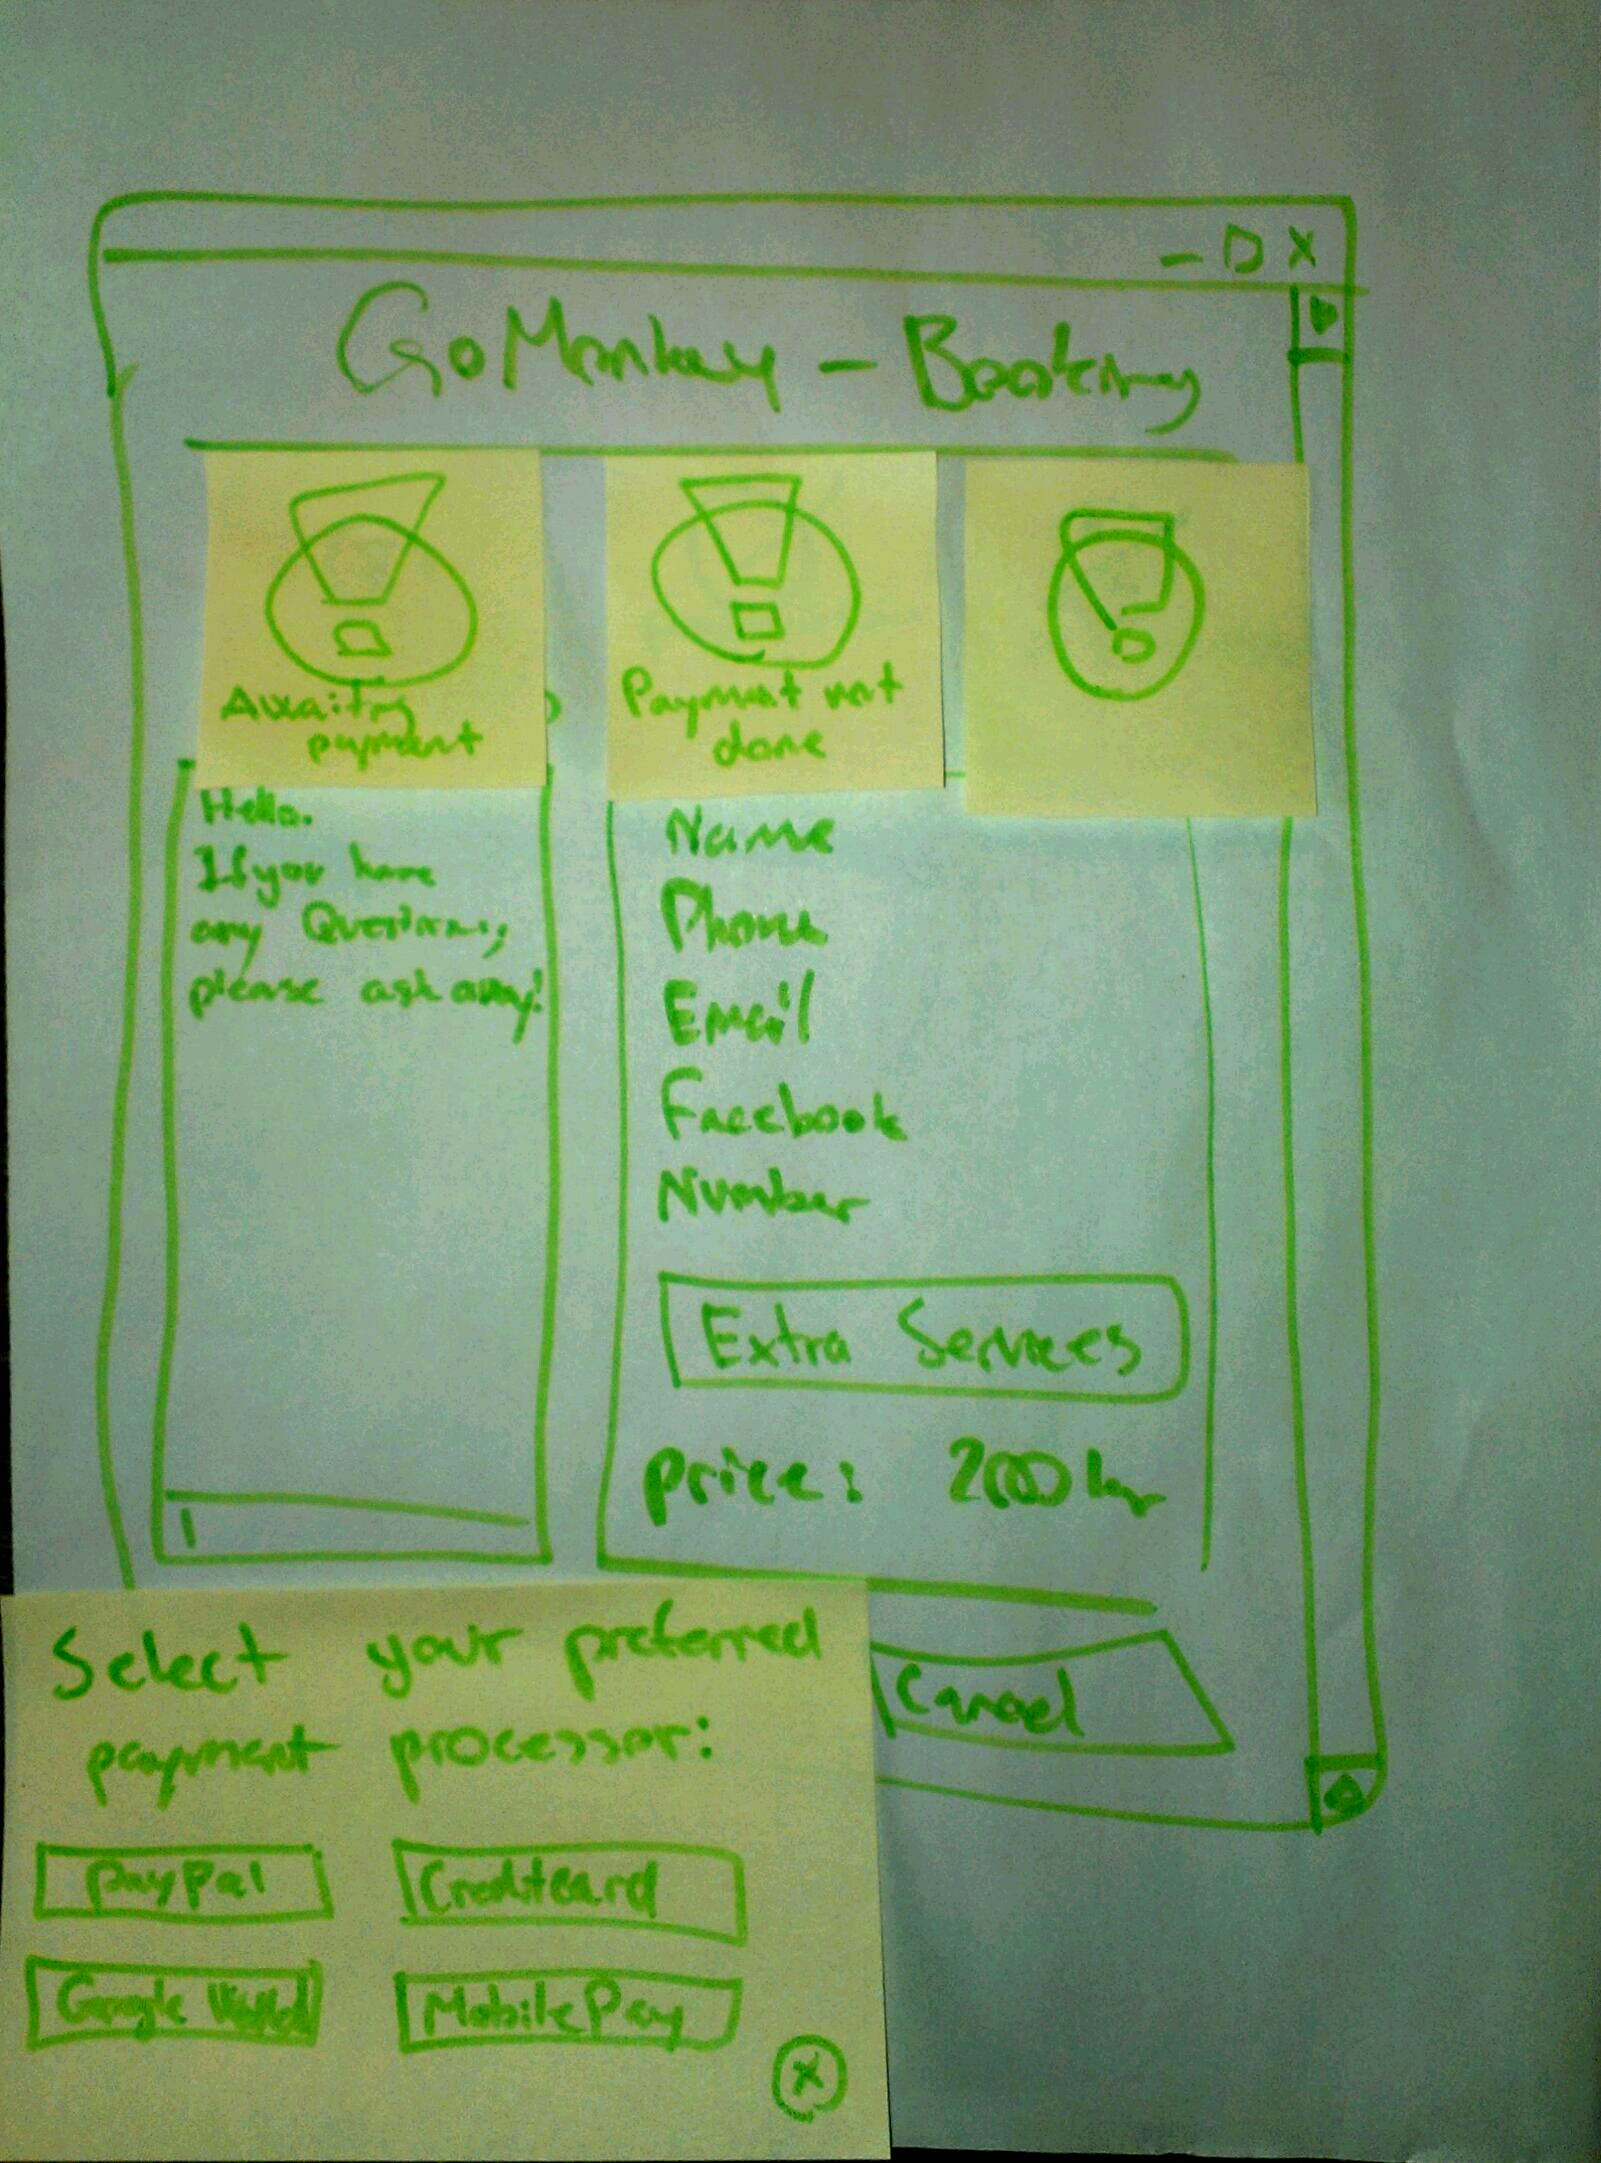
\includegraphics[width=\textwidth]{figures/mockup1}
    \caption{The very first mockup of a booking form. \label{fig:first_mockup}}
\end{figure}

Two parallel tasks were set into motion during the innovation phase: the
development of a set of mockups to represent what a \textit{custom-built system}
could look like, as well as a market study of existing standard systems
available. Aligning the market study against the prioritized goals for the
coherent vision of a new IT system for booking allowed the design team to
primarily discard standard systems, on the grounds of being tailored to a
completely different market. For instance, many booking systems contain a notion
of fixed services, fixed time slots or similar. This clashes with the fluid
booking that \gomonkey{} supports, where a customer can bring \textbf{X}
participants of different ages, at some user-specified time. An experimentation
with a horizontal prototype, the mockups, was performed in-situ with the manager
Michel. This leadi to a large number of suggested changes to the mockups, the uncovering of
additional usecases and edge conditions as well as new knowledge that was not obtained
during the in-depth analysis phase.

Based upon this new knowledge, the mockups created were re-drafted into their
fourth official revision. \autoref{fig:first_mockup} shows the very first drawn
mockup. It is noteworthy that the mockups have changed less
and less each time, perhaps because the problem domain has become more
well-described in each iteration and changes have gone from being large,
sweeping alterations to the overall workflow and over to cosmetic nit-picking.

The mockups became the basis for a vision, which suggests the implementation of
a custom-built system and describes the resources required, the organizational
changes, the skills required by employees and a specific strategy elaborating on
the \textit{why} and \textit{how}.

\reflection{}
%%%%
\begin{description}
    \item [Customer groups] The experimentation with the horizontal prototype unveiled that 
        \gomonkey{} has three primary customer groups: private persons, companies and public
        institutions. For public institutions, a special invoice must be filled
        out by \gomonkey{} which requires obtaining \textit{EAN}-related details
        from the institution, which is an entirely different flow of events from
        how \gomonkey{} usually handles the payment of bookings, i.e.\ through
        looking at bank statements. 
    \item [Altered workflow] The customer booking workflow of the proposed mocked up 
        system was found to be confusing by the Manager, warranting a fundamental change 
        to the way information was passed back and forth between company and customer, 
        to conform more with the way many online websites support purchase of goods and 
        subsequent confirmations. This could be construed as the company wanting
        \textit{less} innovation, or as a pre-existing stereotype interfering
        with the possibility of innovation. A different option is that the
        original flow was simply bad.
\end{description}

\section{A detailed look at some key choices and techniques} \label{sec:detailed}
\subsection{Combining the in-depth and innovation phases}

%\todo[inline]{Describe how we combined the in-depth and
%innovation phases, and how the literature also supports
%this in certain cases. Start by explaining why you would, then explain how we
%did it, then what it gave us. 2-3 pages}

The course allowed combining the ethnographically inspired analysis performed in the
in-depth analysis with the innovation phase due to requesting the results from 
both phases in a single delieverable. Initially, a skeptical approach to the
idea of combining the two phases was taken. We had a \textit{good perception} of the 
work practices after performing the ethnographically inspired analysis, and did not expect
to encounter any new knowledge useable in the in-depth analysis, while performing the 
innovation phase. This assumption was \textit{wrong}, however.
The knowledge gained in the in-depth analysis phase turned out
to be \textit{insufficient}. This resulted in new knowledge being
acquired during the innovation phase, which did not align with the current 
ethnographically inspired analysis and it therefore needed to be \textit{re-adjusted} to be incorporated 
into the way the design team viewed 
\gomonkey{} as a company, and the necessary features of the booking system.

We were not prepared for this discovery, since the material in 
\cite{bodker2004participatory} clearly seperates the in-depth analysis and the 
innovation phase. While it may appear as a utopia to have an ethnographically inspired analysis
that fully describes the actual and true work practices of a company, the course 
material seems to ignore this. It is arguably due to the implicit soft border
between the phases which allows for reworking the results of a previous phase with
newfound knowledge from a later phase.

Realising that the iterative nature of the innovation phase can yield knowledge that
will affect the ethnographically inspired analysis can lead to an increased 
awareness of this possible situation. We suggest that this can help the design team 
continue from a situation where the method doesn't clearly define how to best
utilize the newfound knowledge.

After we became aware how we could utilize the knowledge gained in the innovation 
phase, we returned to the result from the in-depth analysis and reworked the 
suggestions on which the innovation phase was based. This created a more direct
connection of how the results from the innovation phase were based on the 
results of the ethnographically inspired analysis. Had we not returned to the previous
result, we would have had a hard time establishing a clear connection between the 
resulting system and the premisis it was designed upon. Having gone back, we instead 
could point directly to the reason for the design decisions.

\subsection{Ethnographically inspired analysis}
In ethnography, the idea is to immerse yourself in the culture of a
society in order to gain a deeper understanding of the \textit{why}. An
important aspect of this is the realization that the way an activity is explained by an
individual can differ from the actual behavior exhibited when performing that
activity. This has the obvious implication that we must not only hear
descriptions of an activity, but also observe it in action\cite{simonsen1997using}.

This concept is relevant not only in sociological or ethnographic studies, but also if
you perceive a workplace as a culture and environment. This idea has emerged more in recent
years as part of participatory design\cite{crabtree1998ethnography}, perhaps as an attempt to
prevent so-called `tunnel-vision', during which perfect technological solutions are created for
the \textit{wrong} set of problems\cite{sol1984prototyping}. One proposed solution is to pay much
attention to the social organisation of the current 
practice\cite{hughes1994moving, crabtree1998ethnography, simonsen1997using, bodker2004participatory}.

For example, \cite{simonsen1997using} presents a project case involving a film
studio, during which an ethnographically inspired analysis is utilized to
uncover what turns out to be a very complex series of dependencies within the
work organization, to the mutual surprise of both the design team \textbf{and}
the company. \cite{simonsen1997using} surmise that using ethnographically inspired techniques
resulted in changes that challenged the original plan and design, which was developed without.
Needs were uncovered through the ethnographic techniques, that neither designers nor
the film company knew were present.

Surprisingly, \cite{kujala2003user} describes participatory design but specifically separates it from
ethnography as different streams of research, attributing observations and video-analysis to ethnography 
alone, categorizing participatory design by an emphasis on democratic participation and techniques revolving 
around workshops and prototypes. This is in disagreement with \cite{bodker204participatory}, in which
observations and interviews are \textbf{central} techniques and ethnography plays an inclusive, important role.

Despite disagreements over which areas overlap how, it seems a general trend that work in the IT industry consider
ethnographic approaches more and more, as models of a work environment continue to improve and encompass more diverse
situations. The virtue of pursuing this angle can easily be seen by considering the reports of The Standish Group, where
factors that can easily be related to ethnographically quantifiable concepts continue to be top factors in successful IT
projects to this\cite{standish2012}.

For these reasons, particular attention was paid to techniques that would uncover the underlying \textbf{reasons} for
the current work practices at \gomonkey{} during the in-depth analysis and innovation phases. In line with relevant
articles mentioned above, many things were discovered during observations and interviews, which had not surfaced earlier
in more direct, prompted queries about work process. However, it is important to be aware of the \textbf{limitations} of
these ethnographically inspired techniques as well. An observation only observes what the observed happens to be doing, and
does not capture activities that lie outside of the observation. This may seem like an obvious tangent, but it is easy to fall
into a trap of thinking that you have covered all bases because you have done rigorous observation or interviews. Corner cases
are quite often defining for work practice and can sometimes be very hard to capture during observation, especially if neither
the company or design team are acutely aware of their existence.

%\subsection{User stories as a technique}
%\todo[inline]{Describe how user stories work as a technique
%to provide overview and structure workflow. Describe how we
%performed this and provide relevant sources for others who
%use user stories to case out design or implementation of
%projects. Describe some of the pitfalls. Briefly cite and
%describe one alternative to user stories. 1-2 pages}
